
\documentclass[ms.tex]{subfiles} 
\begin{document} 

\section{Nucleosynthesis} 
\label{sec:yields} 

\begin{itemize} 
	\item Although we're computing abundances for N, O, and Fe in the present 
	paper, O and Fe were already explored in detail by~\citet{Johnson2021}, and 
	we retain their parameterization of O and Fe supernova yields here. 
	As required by~\vice, the supernova yields are defined as the net mass of 
	some element X produced over all explosion events in units of the 
	progenitor star cluster's mass. 
	For example, with a yield of~$y_\text{X}$ = 0.001, a 1000~\msun~cluster 
	would produce 1~\msun~of the element X instantaneously in the case of 
	CCSNe or over the delay time distribution (DTD) in the case of SNe Ia. 
	We take the following values from~\citet{Johnson2021}, who in turn base 
	them off of~\citet{Weinberg2017} and~\citet{Johnson2020}: 
	\begin{itemize} 
		\item $y_\text{O}^\text{CC}$ = 0.015 

		\item $y_\text{Fe}^\text{CC}$ = 0.0012 

		\item $y_\text{O}^\text{Ia}$ = 0 

		\item $y_\text{Fe}^\text{Ia}$ = 0.00214 
	\end{itemize} 

	\item We set~$y_\text{N}^\text{Ia}$ to zero and spend the remainder of this 
	section detailing our CCSN and AGB star yields of N. 
\end{itemize} 

\subsection{Core Collapse Supernovae and Massive Star Winds} 
\label{sec:methods:ccsn} 

\begin{figure*} 
\centering 
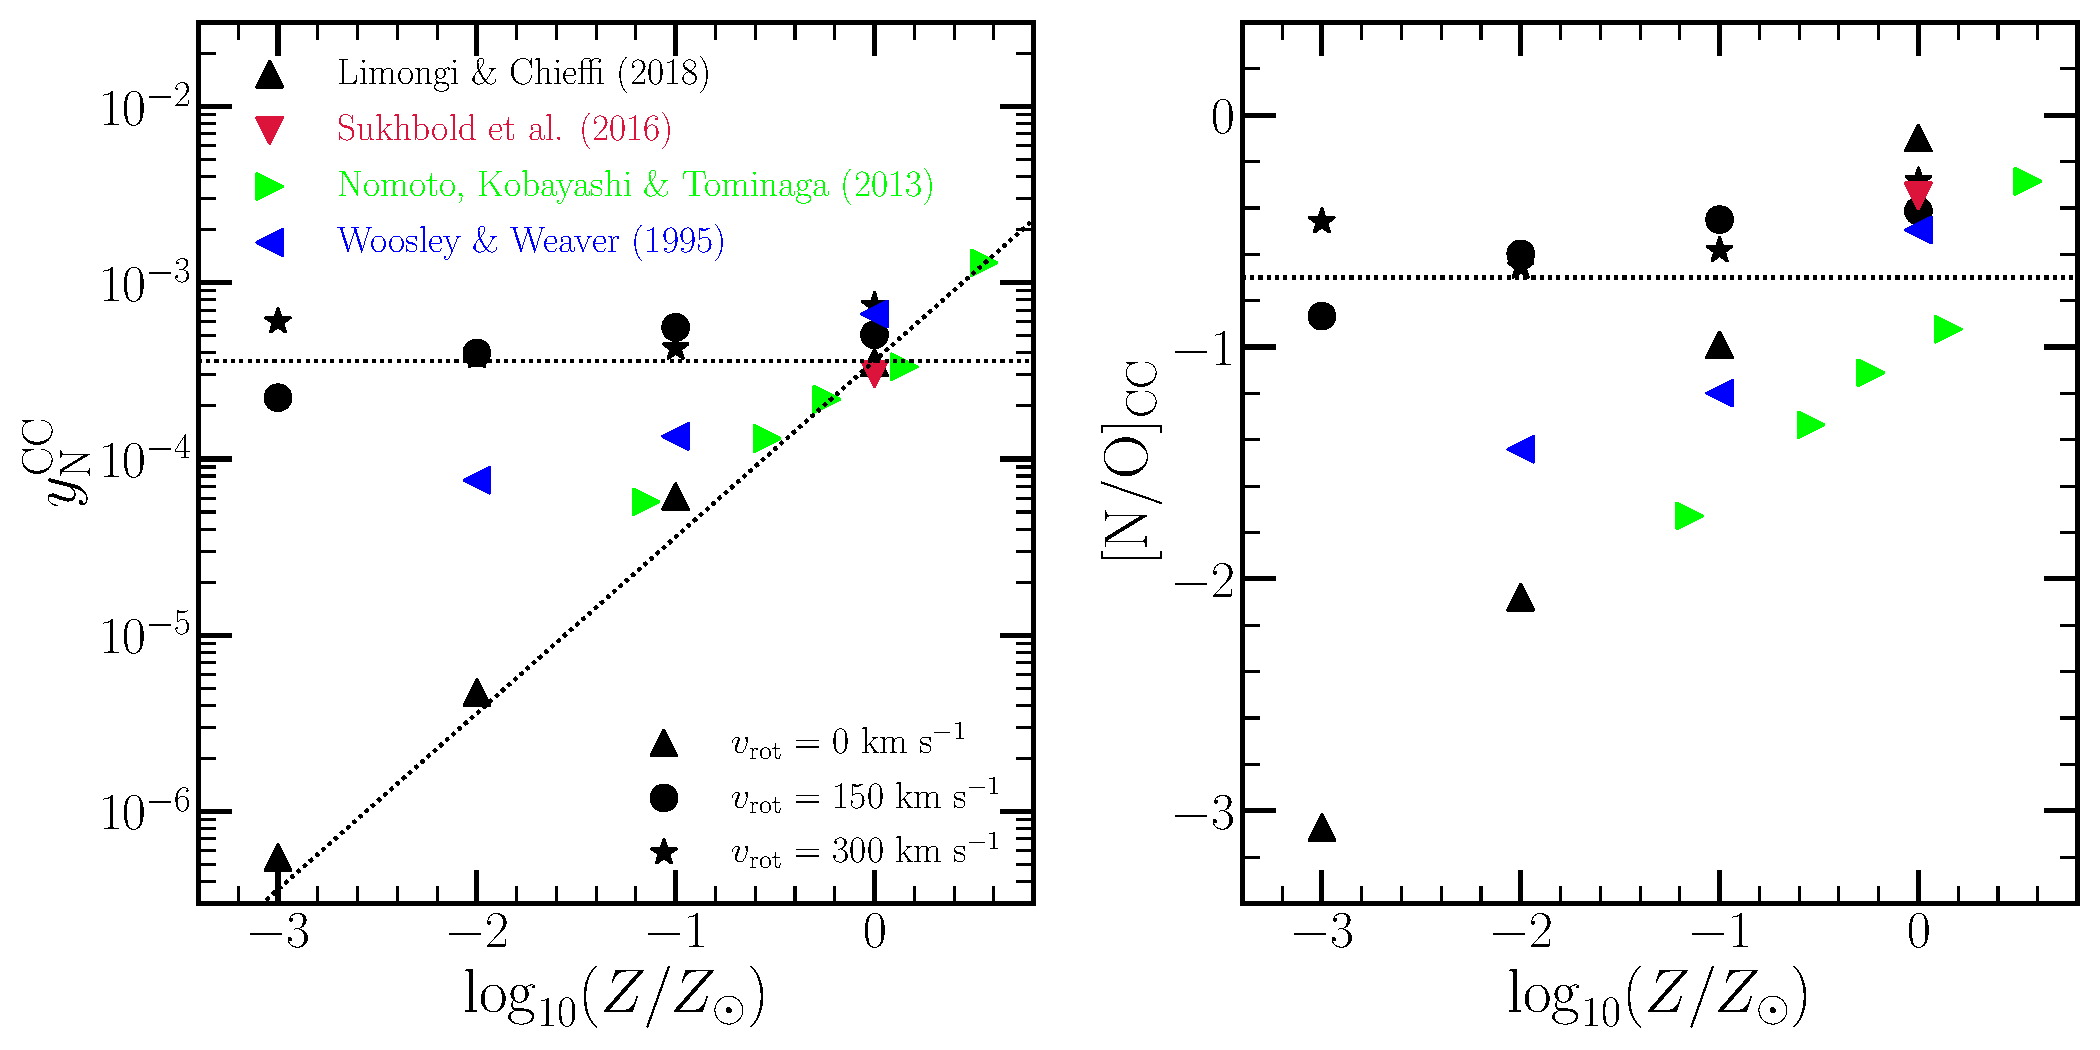
\includegraphics[scale = 0.5]{n_cc_yields.pdf} 
\caption{
\textbf{Left}: IMF-averaged CCSN yields of N calculated 
using~\vice's~\texttt{vice.yields.ccsne.fractional} function with the tables 
published by~\citet[][blue]{Woosley1995},~\citet*[][green]{Nomoto2013}, 
\citet[][red]{Sukhbold2016}, and~\citet[][black]{Limongi2018}. 
All studies report yields for non-rotating progenitors only with the exception 
of~\citet{Limongi2018}, who also report yields for progenitor rotational 
velocities of 150 (triangles) and 300 km/s (stars). 
\textbf{Right}: The~\no~ratio predicted by each of the explosion models in 
the left-hand panel, under the same colour-coding and marker scheme. 
We mark the position of~\no~= $-0.7$ with a black dotted line, the value 
roughly suggested by the observations of low-metallicity systems highlighted in 
Fig.~\ref{fig:no_oh_observed}. 
}
\label{fig:n_cc_yields} 
\end{figure*} 

\begin{itemize} 
	\item In~\vice, CCSN nucleosynthetic products are approximated to be 
	produced instantaneously following an episode of star formation; this is a 
	valid approximation due to how short the lives of massive stars are 
	compared to the relevant timescales for GCE. 
	The yield is the constant of proportionality between the CCSN production 
	rate and the SFR: 
	\begin{equation} 
	\dot{M}_\text{X}^\text{CC} = y_\text{X}^\text{CC}\dot{M}_\star. 
	\end{equation} 
	More generally,~$y_\text{X}^\text{CC}$ quantifies~\textit{all} of the 
	nucleosynthetic material approximated to be produced instantaneously 
	following a single stellar population's formation, though the majority of 
	such events will be associated with massive stars and their supernovae. 
	In the case of N specifically, a substantial amount emerges in winds before 
	the actual supernova explosion itself, allowing massive stars to produce 
	a lot of N even if they collapse directly to a black 
	hole~\citep{Griffith2021}. 

	\item We compute theoretically predicted values of~$y_\text{N}^\text{CC}$ 
	assuming a~\citet{Kroupa2001} IMF using~\vice's 
	\texttt{vice.yields.ccsne.fractional} function; details on how~\vice~handles 
	these calculations can be found in~\S~4 of~\citet{Griffith2021} and in 
	the~\vice~science documentation.\footnote{
		\url{https://vice-astro.readthedocs.io/en/latest/science_documentation/yields/index.html} 
	}
	The left panel of Fig.~\ref{fig:n_cc_yields} plots the results as a 
	function of progenitor metallicity predicted by the~\citet{Woosley1995}, 
	\citet{Nomoto2013},~\citet{Sukhbold2016}, and~\citet{Limongi2018} tables. 

	\item There is good agreement between the various non-rotating models, but 
	only~\citet{Limongi2018} report yields for progenitors with a non-zero 
	rotational velocity. 
	These yields are substantially larger than that of their non-rotating 
	counterparts. 
	Most of the N production in CCSN progenitors occurs via the CNO cycle 
	processing C and O isotopes into~\Nfourteen, and with few C and O seed 
	nuclei at low~$Z$, production of~\Nfourteen~is difficult. 
	Rotationally induced mixing, a highly uncertain process~\citep{Zahn1992, 
	Maeder1998, Lagarde2012}, could transport newly produced C and O into the 
	hydrogen burning shell of the CCSN progenitor, facilitating N production 
	(\citealp{Frischknecht2016}; see also discussion in~\S~4.2 
	of~\citealp{Andrews2017}). 
	For this reason, N yields at low metallicity are quite sensitive to these 
	assumptions about stellar rotation and internal mixing 
	processes~\citep{Heger2010}, and consequently IMF-averaged yields are 
	highly uncertain. 

	\item Based on the definition of the abundance ratio [X/Y], we can compute 
	the [N/O] ratio of CCSN ejecta from the values of~$y_\text{N}^\text{CC}$ 
	and~$y_\text{O}^\text{CC}$: 
	\begin{equation} 
	\text{[N/O]}\subcc = 
	\log_{10}\left(
	\frac{y_\text{N}^\text{CC}}{y_\text{O}^\text{CC}}
	\right) 
	- \log_{10}\left(
	\frac{Z_{\text{N},\odot}}{Z_{\text{O},\odot}}
	\right) 
	\label{eq:no_cc} 
	\end{equation} 
	where~$Z_{\text{X},\odot}$ is the abundance by mass of some element X in the 
	sun. 
	For each of the studies and rotational velocities in the left panel of 
	Fig.~\ref{fig:n_cc_yields}, we compute the corresponding values 
	of~$y_\text{O}^\text{CC}$ using~\vice, and we plot the resultant values of 
	[N/O]\subcc~in the right panel assuming 
	$Z_{\text{N},\odot} = 6.91\times10^{-4}$ and 
	$Z_{\text{O},\odot} = 5.7\times10^{-3}$ based on the solar photospheric 
	abundances of~\citet{Asplund2009}. 
	The resultant values of [N/O]\subcc~follow similar trends with progenitor 
	metallicity and rotational velocity as~$y_\text{N}^\text{CC}$, a 
	consequence of the fact that these studies predict relatively 
	metallicity-independent O yields. 

	\item At low [O/H], the mean~\no~is near~$-0.7$ (see 
	Fig.~\ref{fig:no_oh_observed}). 
	Since the AGB star yields of N are believed to increase with metallicity 
	(e.g.~\citealp{Cristallo2011, Cristallo2015, Ventura2013}), this is likely 
	the regime in which N yields are dominated by CCSN enrichment. 
	We therefore take~\no\subcc~=~$-0.7$ empirically, and we highlight 
	this value in the right panel of Fig.~\ref{fig:n_cc_yields} with a 
	horizontal black dashed line. 
	Given this result, we use equation~\refp{eq:no_cc} with our adopted value 
	of~$y_\text{O}^\text{CC} = 0.015$ and the solar abundances 
	from~\citet{Asplund2009} to compute an empirical value 
	of~$y_\text{N}^\text{CC} = 3.6\times10^{-4}$. 
	We adopt this value as our fiducial CCSN yield of N and highlight it with 
	a horizontal black dashed line in the left hand panel of 
	Fig.~\ref{fig:n_cc_yields}. 
	We discuss the sloped dotted line in that panel in the context of some of 
	our AGB star yield models in~\S~\ref{sec:results:yields}. 

	\item These empirical values of [N/O]\subcc~and~$y_\text{N}^\text{CC}$ are 
	in good agreement with the rotating CCSN models of~\citet{Limongi2018}. 
	This supports the recent argument by~\citet*{Grisoni2021} that rotating 
	massive stars play an important role in establishing the N abundances 
	observed at low metallicities in the Milky Way. 
	Although the~\citet{Sukhbold2016} tables agree nearly perfectly with our 
	empirical value of~$y_\text{N}^\text{CC} = 3.6\times10^{-4}$, they 
	overestimate [N/O]\subcc~by~$\sim$0.2 dex; this is because they predict 
	a value of~$y_\text{O}^\text{CC}$ lower than our adopted value of 0.015. 

	\item Although most of the supernova models plotted in 
	Fig.~\ref{fig:n_cc_yields} slightly overestimate our empirical value of 
	[N/O]\subcc~=~$-0.07$, they're still sub-solar. 
	This implies a need for an additional enrichment channel, as expected 
	because it is well-understood that N is also produced in AGB 
	stars~\citep{Johnson2019}. 
\end{itemize} 

\subsection{Asymptotic Giant Branch Stars} 
\label{sec:methods:agb} 

\begin{figure*} 
\centering 
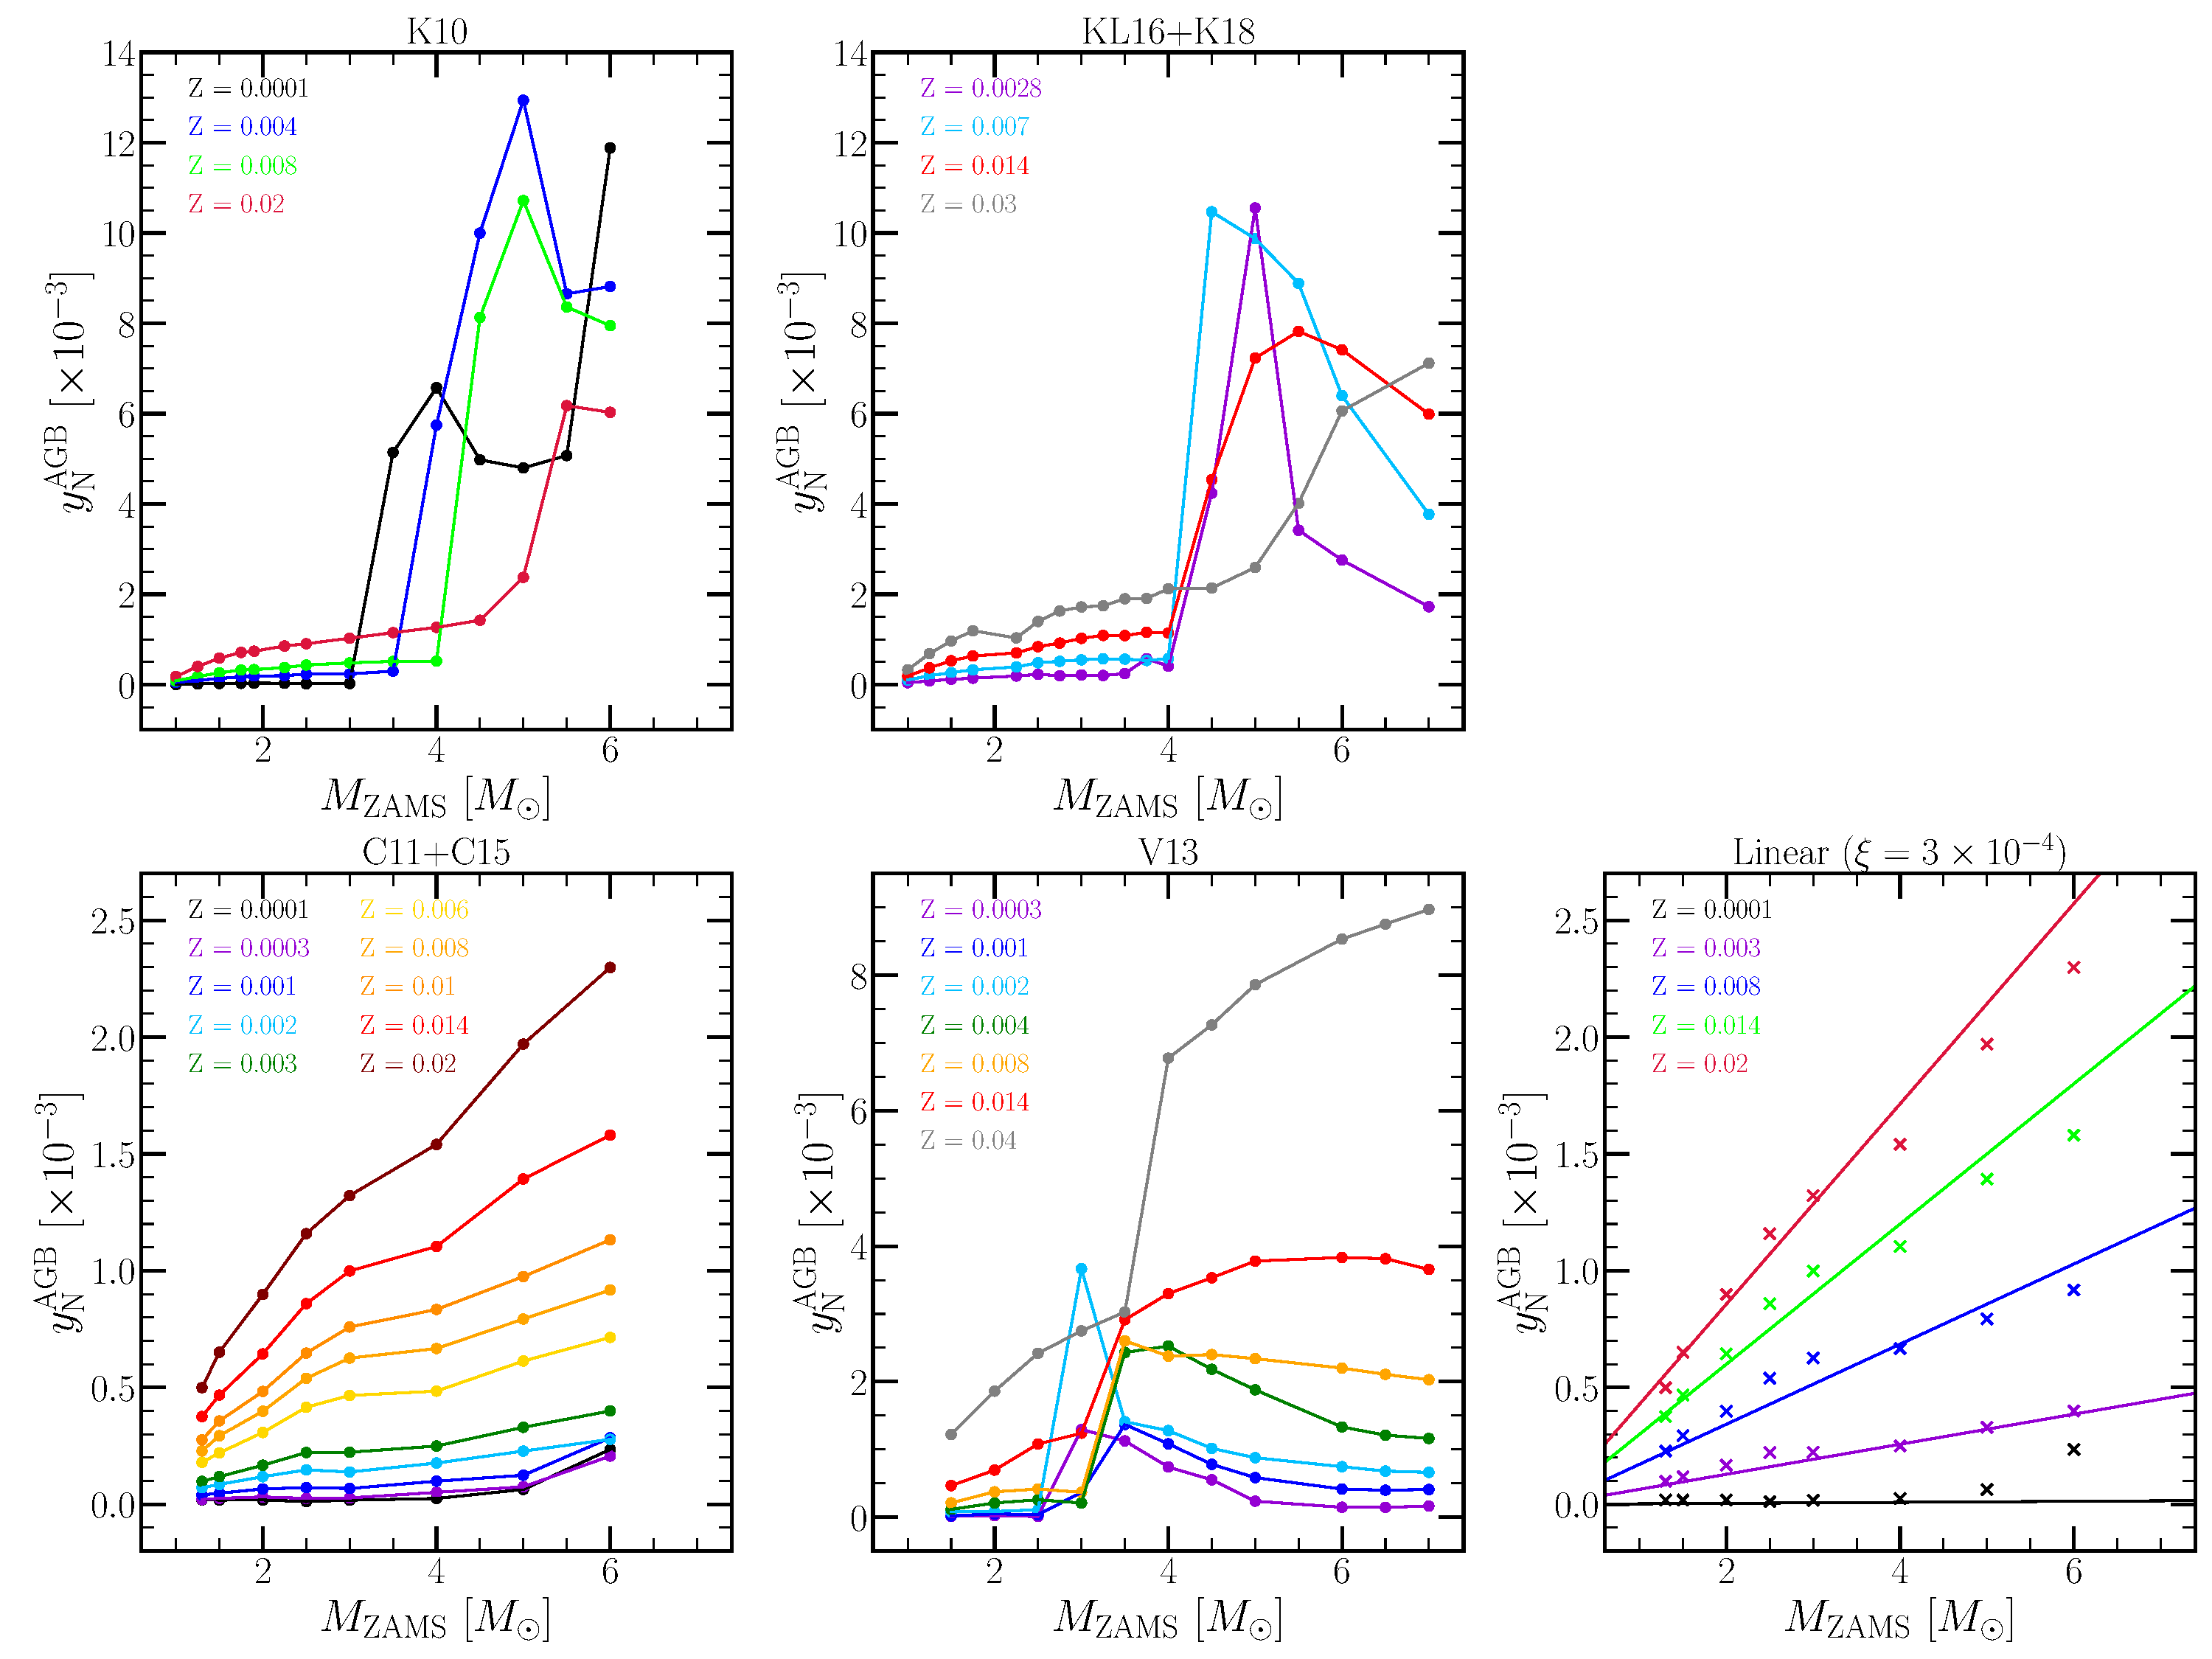
\includegraphics[scale = 0.33]{agb_yield_models.pdf} 
\caption{
The fractional yields of N from AGB stars~$y_\text{N}^\text{AGB}$ as a function 
of progenitor ZAMS mass and birth metallicity~$Z$ as reported 
by~\citet{Karakas2010} (upper left),~\citet{Karakas2016} and~\citet{Karakas2018} 
(upper middle),~\citet{Cristallo2011, Cristallo2015} (lower left), 
and~\citet{Ventura2013} (lower middle). 
In the lower right panel, we show the yields predicted by our linear model 
(colored lines; see discussion in~\S~X) in comparison to 
the~\citet{Cristallo2011, Cristallo2015} predictions (colored X's). 
}
\label{fig:agb_yield_models} 
\end{figure*} 

\begin{itemize} 
	\item In the present paper, we're interested in the question of how 
	well the ``off the shelf'' AGB star yield models for N can reproduce the 
	observed [N/O]-[O/H] relation. 

	% \item {[As discussed in~\S~\ref{sec:intro},]} the majority of nitrogen 
	% production occurs through the CNO cycle, the slowest component of which is 
	% the~\Nfourteen(p,$\gamma$)\Ofifteen~reaction which produces a bottleneck, 
	% effectively turning all of the different C, N, and O isotopes 
	% into~\Nfourteen. 

	\item Similar to the SN yields (see discussion above), these are defined as 
	fractional net yields in that they quantify only the newly produced N in 
	the AGB star ejecta in units of its ZAMS mass. 
	For a yield~$y_\text{N}^\text{AGB}(M_\star, Z_\star)$, the actual mass 
	yield is then given by~$M_\star y_\text{N}^\text{AGB}(M_\star, Z_\star)$. 
	AGB star enrichment proceeds as it does in~\citet{Johnson2020} under the 
	caveat that the yield is placed in the~$\delta\rgal$ = 100 pc ring that a 
	stellar population is in at a given time. 
	In short,~\vice~implements an algorithm which calculates the mass in dying 
	stars from each previous star formation event (i.e. timestep), and the ZAMS 
	mass required to calculate the yield comes from a mass-lifetime 
	relation (e.g.~\citealp{Larson1974, Maeder1989, Padovani1993, Kodama1997}; 
	\citealp*{Hurley2000};~\citealp{Vincenzo2016b}). 

	\item In the present paper, we make use of four previously published sets 
	of AGB star yields calculated from stellar evolution models, each of which 
	are sampled on a table of progenitor masses and metallicities: 

	\begin{itemize} 
		\item The default set of yields is published 
		in~\citet[][hereafter~\cristallo]{Cristallo2011, Cristallo2015}. 
		We illustrate these yields as a function of ZAMS mass for the available 
		metallicities in the lower left panel of 
		Fig.~\ref{fig:agb_yield_models}. 
		This is the most comprehensive set of yields in~\vice~in that it 
		includes tables for all elements built into the code and is sampled at 
		the most metallicities.  

		\item The~\citet[][hereafter~\karakasten]{Karakas2010} is plotted in 
		the upper left panel of Fig.~\ref{fig:agb_yield_models}. 

		\item The~\citet[][hereafter~\ventura]{Ventura2013} yields are 
		illustrated in the bottom middle panel of 
		Fig.~\ref{fig:agb_yield_models}. 

		\item We combine the yields published in~\citet{Karakas2016} 
		at~$Z = 0.007$, 0.014, and 0.03 with those published 
		in~\citet{Karakas2018} at~$Z = 0.0028$; we hereafter refer to these 
		tables as the~\karakas~set of yields. 
		We plot them in the upper middle panel of 
		Fig.~\ref{fig:agb_yield_models}. 
	\end{itemize} 

	\item {\color{red} To do: Add an appendix on all of the stuff that's new 
	to~\vice~with this paper?} 

	\item \vice~also allows users to construct their own functions of 
	progenitor mass and metallicity to describe the AGB star yield. 
	Motivated by the roughly linear nature of the~\cristallo~yields and their 
	general success once renormalized by a constant factor (see discussion 
	in~\S~\ref{sec:results}), we construct a model in which the yield is 
	linearly proportional to both progenitor ZAMS mass and metallicity 
	according to: 
	\begin{equation} 
	y_\text{N}^\text{AGB} = \xi\left(\frac{M}{M_\odot}\right) 
	\left(\frac{Z}{Z_\odot}\right) 
	\label{eq:linear_yield} 
	\end{equation} 
	We illustrate this model in the lower right panel of 
	Fig.~\ref{fig:agb_yield_models} for~$\xi = 3\times10^{-4}$ in comparison to 
	the~\cristallo~yields shown by the coloured X's. 
\end{itemize}

\begin{figure*} 
\centering 
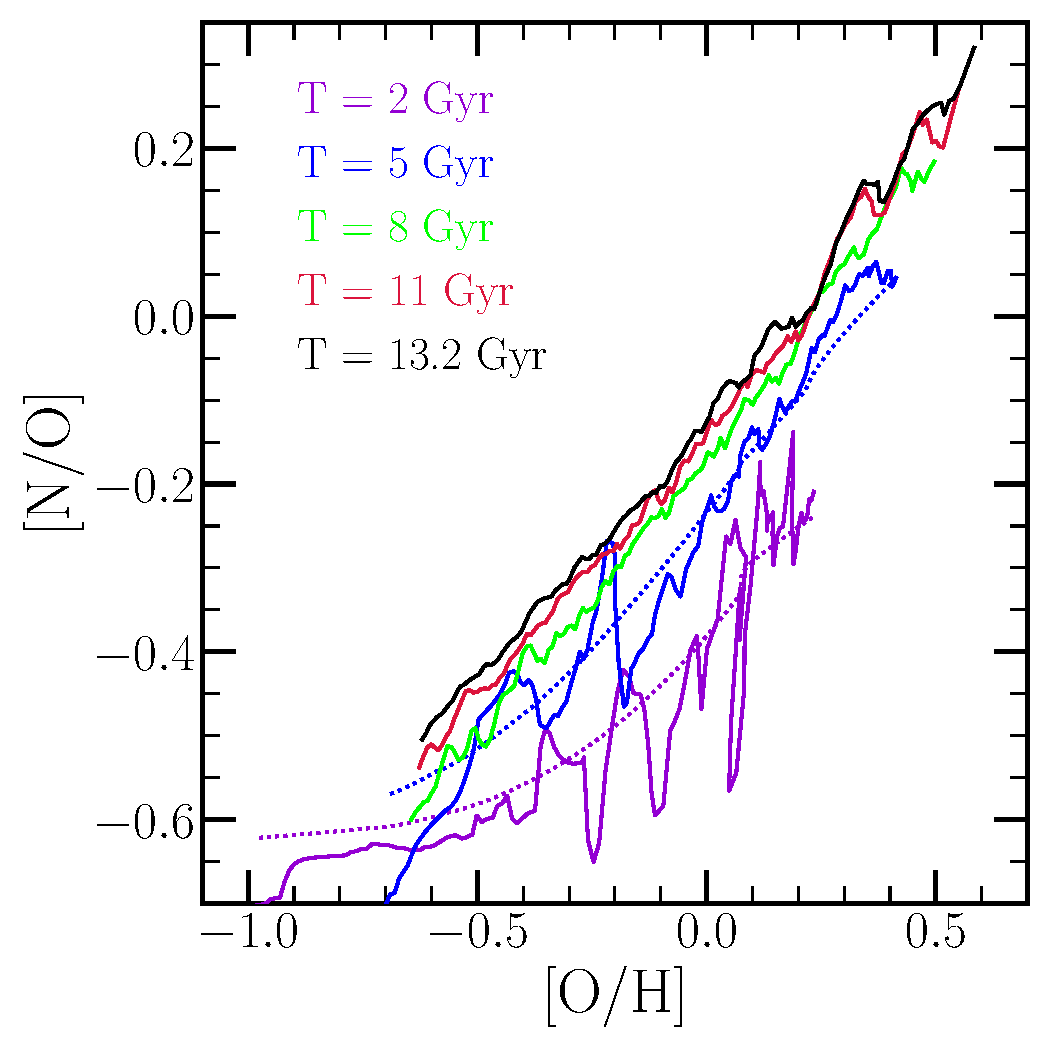
\includegraphics[scale = 0.45]{no_oh_timeevol.pdf} 
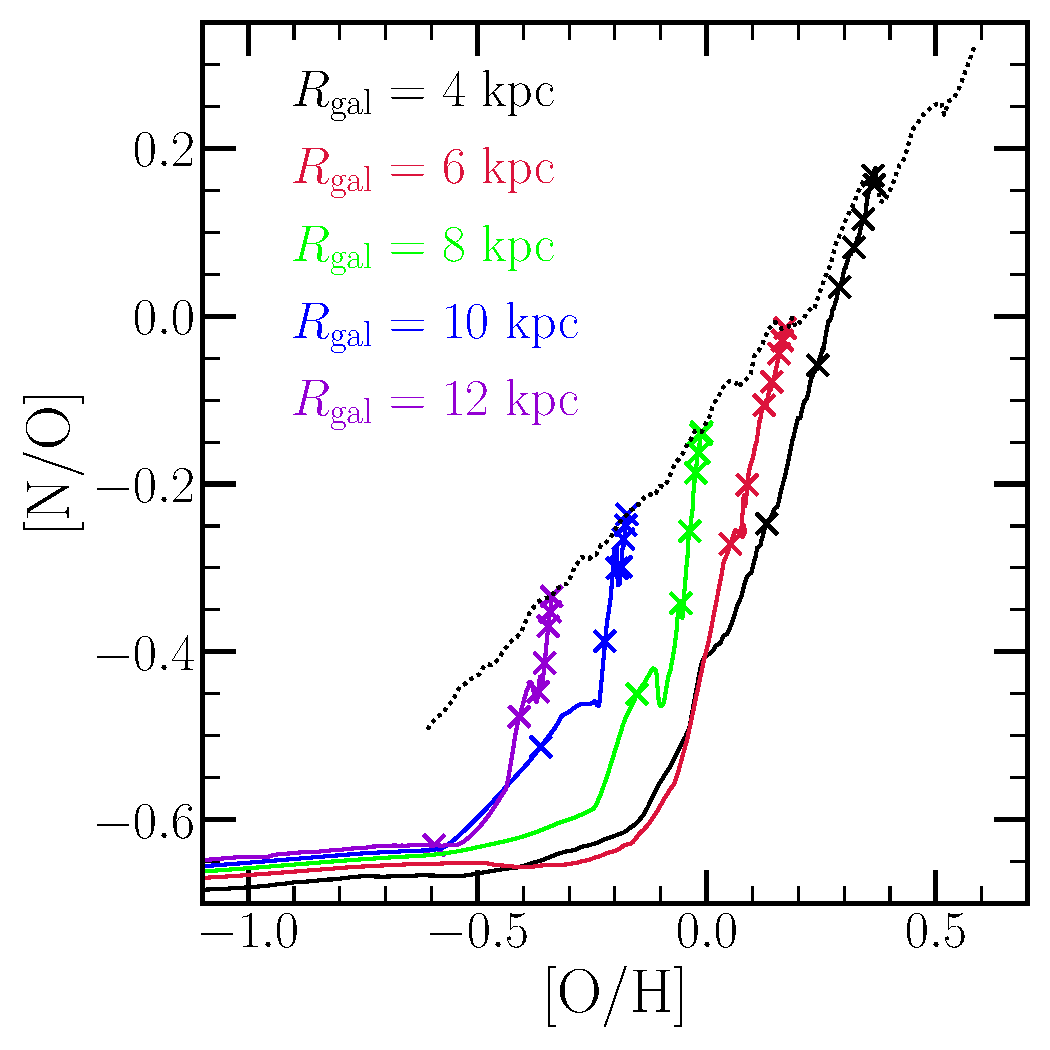
\includegraphics[scale = 0.45]{no_oh_superposition.pdf} 
% 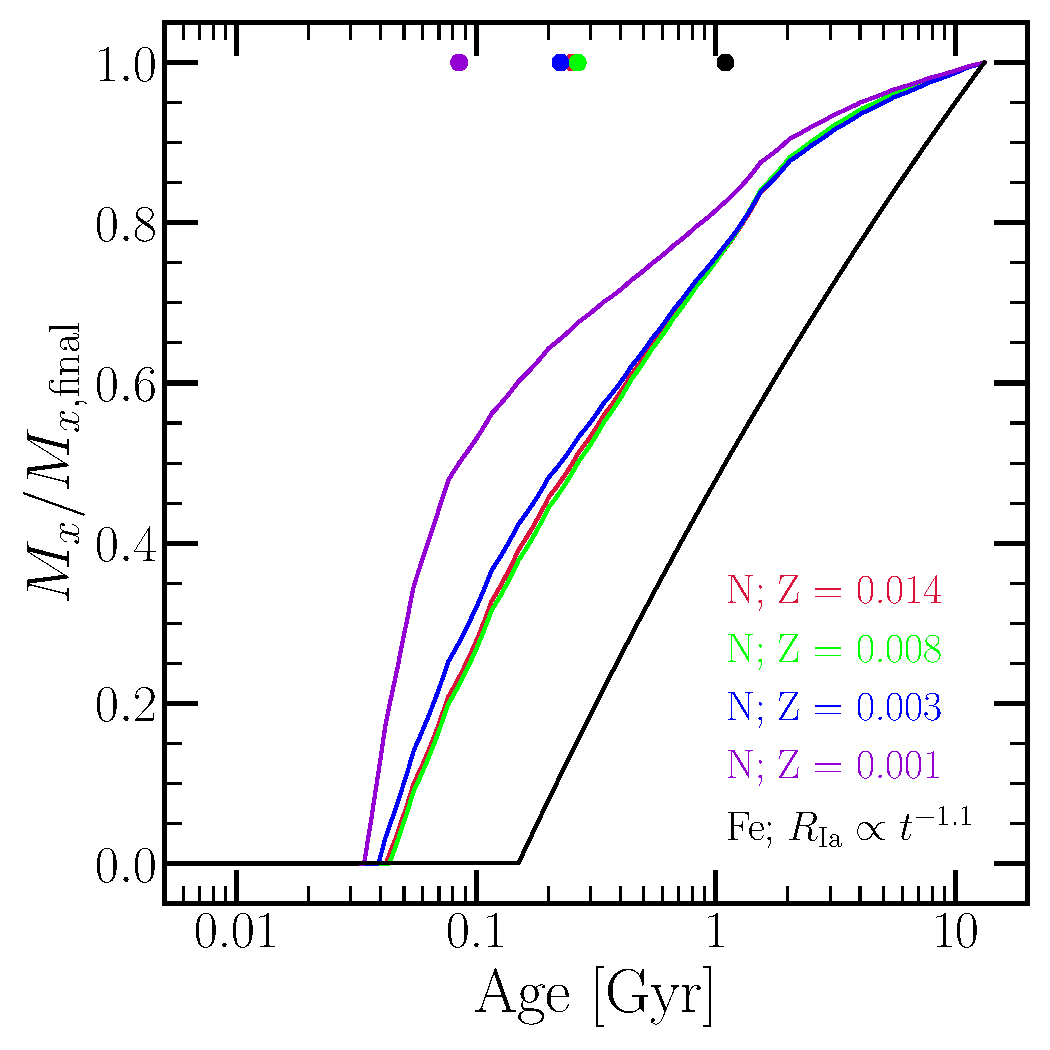
\includegraphics[scale = 0.3]{ssp_production.pdf} 
\caption{
\textbf{Left}: The gas-phase [N/O]-[O/H] relation parameterized by radius at 
various snapshots (solid coloured lines) in our fiducial model with 
the~\cristallo~yields. 
Dotted lines denote the resulting relation at~$T$ = 2 and 5 Gyr in the model 
where we neglect stellar migration. 
\textbf{Right}: The gas-phase [N/O]-[O/H] relation parameterized by time at 
fixed radius (solid coloured lines) in the fiducial model. 
X's denote the abundances at~$T$ = 2, 4, 6, 8, 10, 12, and 13.2 Gyr (the 
present day) at these radii. 
The dotted line is the same as the solid black line in the left hand panel. 
} 
\label{fig:no_oh_timeevol} 
\end{figure*} 

\begin{itemize} 
	\item Despite reporting values of the same physical quantities, the N 
	yields reported by each of these studies show substantial differences 
	between one another. 
	Unforunately, ascertaining the origins of these differences is difficult 
	because each study employs different assumptions for mass loss, nuclear 
	reaction networks, and convection and convective boundaries within the 
	star, all of which have a significant impact on stellar evolution and thus 
	the predicted yields (see discussion in, e.g.,~\S~5 
	of~\citealp{Karakas2016}). 
	However, the differences can largely be understood by considering two 
	phenomena known to occur within AGB stars: third dredge-up and hot bottom 
	burning. 
	Collapsing the information into these two processes is helpful because 
	their differences arise as a consequence of the different input physics 
	between the stellar evolution models. 
	\begin{itemize} 
		\item Third dredge-up (hereafter TDU)\footnote{
			Here the time adverbial ``third'' refers only the fact that the 
			star is on the asymptotic giant branch. 
			First dredge-up occurs when a star first ascends the red giant 
			branch, and second dredge-up occurs when the star ends its 
			helium-burning lifetime. 
			Because TDU episodes are associated with thermal pulsations, there 
			are many TDU events during a star's AGB lifetime. 
		} refers to the repeated penetrations of the convective envelope into 
		the hydrogen depleted core during the thermal pulses associated with 
		AGB star evolution.
		This process doesn't affect N abundances much, but replenishes the 
		outer layers of the star with C and O. 
		In low mass AGB stars, the main source of free neutrons is the 
		\Cthirteen($\alpha$,n)\Osixteen~reaction, which can occur at 
		substantial rates when C is mixed with the He-rich shell during each 
		TDU episode. 

		\item Hot bottom burning (hereafter HBB) refers to the activation of 
		proton captures at the base of the convective envelope activating the 
		CNO cycle and producing large amounts of~\Nfourteen~at the expense of C 
		and O isotopes. 
		HBB requires a higher mass AGB star progenitor ($\sim$4 - 5~\msun at 
		Z$_\odot$) than TDU ($\sim$2 - 2.5~\msun at Z$_\odot$), but the 
		minimum mass for both decreases at lower metallicity. 
	\end{itemize} 

	\item The most efficient N production occurs when both TDU and HBB 
	occur within an AGB star, because each replenishment of C and O 
	isotopes from the core adds new seed nuclei for the CNO cycle when HBB 
	is active. 
	This is the reason for the substantial N production 
	above~$\sim$4~\msun~in the~\karakasten~and~\karakas~models; in both 
	yield sets, every star that experiences HBB also experiences TDU. 
	Both TDU and HBB are more efficient at low metallicity (see discussion 
	in~\ventura). 
	In the case of TDU, each penetration of the convective envelope into 
	the H-depleted core is deeper because of the lower opacity. 
	For HBB, the base of the convective envelope is hotter, increasing the 
	rate of nuclear reactions relative to the higher~$Z$ models. 
	Though there are some exceptions evident in Fig.~\ref{fig:agb_yield_models}, 
	the highest N yields in the~\karakasten~and~\karakas~models are for low 
	metallicity stars above~$\sim$4~\msun for exactly this reason. 

	\item This interaction between TDU and HBB is also the reason for the 
	increase in N yields in the~\ventura~tables near~$\sim$3~\msun. 
	Unlike the~\karakasten~and~\karakas~models, their stars experience 
	both TDU and HBB only in this narrow range in mass. 

	\item Of all of these yields taken from the literature, 
	the~\cristallo~sample shows the smoothest dependence on progenitor mass 
	and metallicity. 
	Unfortunately, ascertaining the exact cause of this difference between 
	the other yields explored here is difficult even when collapsing the 
	information into TDU and HBB; relative to the~\karakas~yields (see 
	discussion in their~\S~5), the~\cristallo~models have more mass loss, 
	a~$\sim$10\% faster triple-$\alpha$ reaction rate, fewer thermal pulses 
	overall, and weaker HBB due to a lower temperature at the base of the 
	convective envelope. 
	Though their agreement is good below~$\sim$3~\msun, the fact that 
	HBB is weaker and fewer TDU episodes are experienced does however lend 
	a qualitative explanation into why the~\cristallo~yields are so much 
	smaller than the~\karakasten~and~\karakas~yields at higher masses. 

	\item {\color{red} To do: Comment on the differences between 
	the~\karakasten~and~\karakas~models.} 

	\item In the interest of consistency, when we adopt a particular AGB star 
	yield model for N, we also adopt it for O and Fe when possible.\footnote{
		In the case of the~\ventura~model, AGB star yields of Fe are not 
		available. 
	} 
	However, the AGB star yields of these elements are negligible compared to 
	their supernova yields. 
\end{itemize} 

\end{document} 
